\subsection{Architectures} \slabel{arch}

We run on two supercomputers: Mira at the ALCF and Shaheen XC40 at the KSL.
Mira is a IBM BlueGene/Q with 49,152 nodes.
Each node has 16 cores with 4 hardware threads per core and can support 204.8
GFLOPS and 30 GiB/s main memory bandwidth, measured by~\cite{McCalpin2007}.
Shaheen is a Cray XC40 with 6144 nodes.
Each node has two Intel\textsuperscript{\textregistered}
Xeon\textsuperscript{\textregistered} E5-2698v3 (code-named Haswell) processors
with 16 cores each and can support around 1177.6 GFLOPS and 101.6 GiB/s main memory bandwidth, measured by~\cite{McCalpin2007}.
Shaheen's cores therefore have 2.9$\times$ the floating point and 1.7$\times$ the memory bandwidth of Mira's BlueGene/Q cores.

\subsection{Single mode Rayleigh-Taylor instability}

The Rayleigh-Taylor instability (RTI) occurs when the pressure and density gradients point in opposite directions, as in the canonical case of a heavy fluid supported on top of a lighter fluid in a gravitational field.
The Rayleigh-Taylor growth rate is an increasing function of the wave-number, up to a viscous cutoff, making the smallest scales grow fastest.
Because energy is pumped into the system at small scales, the RTI is notoriously difficult to model numerically~\cite{Dimonte2004}.

The RTI describes how the dense fluid is pushed through and mixes with lighter fluid.
This dynamic mixing process is essential to the behavior of flows found in exploding stars~\cite{Bell2004}, the oceans and atmosphere~\cite{Linden1973}, and inertial confinement fusion.
In the latter case, dense plastic ablator is pushed into and mixed with the lighter hydrogen fuel.
The carbon-laden ablator radiates energy much more quickly than the fuel, reducing hot-spot temperature and preventing ignition.
The study of the RTI and related mixing is a priority research direction for inertial confinement fusion performance~\cite{Gocharov2012}.

Nek5000 and NekBox~\cite{NekBox} are used to model the incompressible Boussinesq equations, which approximate the RTI at low density contrasts:
\begin{align}
\frac{\partial u}{\partial t} + u \cdot \nabla u &= - \nabla p + \nu \nabla^2 u + \tilde{g} T \\
\frac{\partial T}{\partial t} + u \cdot \nabla T &= \alpha \nabla^2 T \\
\nabla \cdot u &= 0,
\end{align}
where $T$ is a scalar that can be interpreted as a temperature, 
in which case $\alpha$ is the thermal diffusivity 
and $\tilde{g}$ is the product of the gravitational acceleration and the thermal expansion coefficient.

The single-mode Rayleigh-Taylor instability (smRTI) restricts the initial perturbation of the interface to be sinusoidal, and is generally considered in periodic span-wise boundary conditions:
\begin{equation} \elabel{IC}
T(x,y,z,0) = A\cdot \text{erf}\left[\frac{z + a_0 \cos(2 \pi x/\lambda) \cos(2 \pi y/\lambda)}{\delta}\right],
\end{equation}
where $A \in (0,1]$ is the Atwood number,
$\lambda$ is the wavelength, 
$a_0$ is the initial interface amplitude, and
$\delta$ is the initial interface width.
This simplification allows the problem to be defined by only two dimensionless numbers in the limit of $a_0, \delta \rightarrow 0$, the Grashof number (Gr) and the Prandtl number (Pr):
\begin{equation}
\text{Gr} = \frac{A \tilde{g} \lambda^3}{\nu^2},  \qquad \text{Pr} = \frac{\nu}{\alpha}.
\end{equation}

Even under these simplifications, the late-time behavior is not well understood.
Experiments are prone to spurious low-wavelength modes that dominate the dynamics at late times, while the cost of direct numerical simulations is quadratic with the domain's aspect ratio.

It would be valuable to systematically sample the Grashof-Prandtl space with high fidelity simulations at late-time/high-aspect-ratio to better inform experimental design and model development.
Such a study would be very expensive, so it is important to select a cost-minimizing strategy.

We take this problem, the selection of a cost-minimizing strategy for the late-time smRTI, as our motivation.
In addition to the isolated reproducers discussed in \sref{implementation}, we present NekBox application benchmarks based on smRTI with typical Nek settings.
The aim of these benchmarks is to identify minimum cost discretizations that attain a given accuracy.

The benchmarks are conducted for combinations of the element size taken from
\begin{equation}
\{4, 6, 8, 10, 12, 14, 16, 32\},
\end{equation}
and span-wise mesh size taken from 
\begin{equation}
\{2, 4, 8, 12, 16, 24, 32, 48, 64, 96, 128\}.
\end{equation}
The total number of points ranges from around 1 million to 4 billion.
The problem is weak-scaled: the number of elements per rank is chosen as to consume approximately half of the available main memory, or around 16k and 262k points per rank on Mira and Shaheen, respectively.
The problems are constrained to fill an integer number of nodes, which puts a lower bound on the mesh size and excludes some cases that would partially fill nodes.
The domain is a box with dimension $[0,0.5]^2 \times [-1,1]$, and the elements are cubic.
The span-wise boundary conditions are symmetric and the vertical boundary conditions are no-slip in velocity and no-flux (insulating) in the scalar.
The initial condition is stationary in velocity with a scalar given by \eref{IC}, the Grashof number is 17,324, and the Prandtl number is 1.
The timestep is calculated based on a Courant number of $0.4$, which scales linearly with the number of elements and quadratically with the size of the element due to the spacing of the GLL nodes.
The Courant condition is defined only in a linear limit, so during the initial exponential growth regime the Courant number is computed using the stagnation velocity, $\sqrt{A \tilde{g}/(\pi \lambda)}$.


Outputs are written at regular intervals in simulated time, constant across problem sizes.
Therefore, smaller problems perform a greater share of I/O, as is the common case in CFD.
Nek5000 and NekBox write separate files for separate ranks.
The number of ranks that participate in I/O is a fixed proportion of the total number of ranks.

\begin{figure}
\begin{subfigure}[b]{0.24\textwidth}
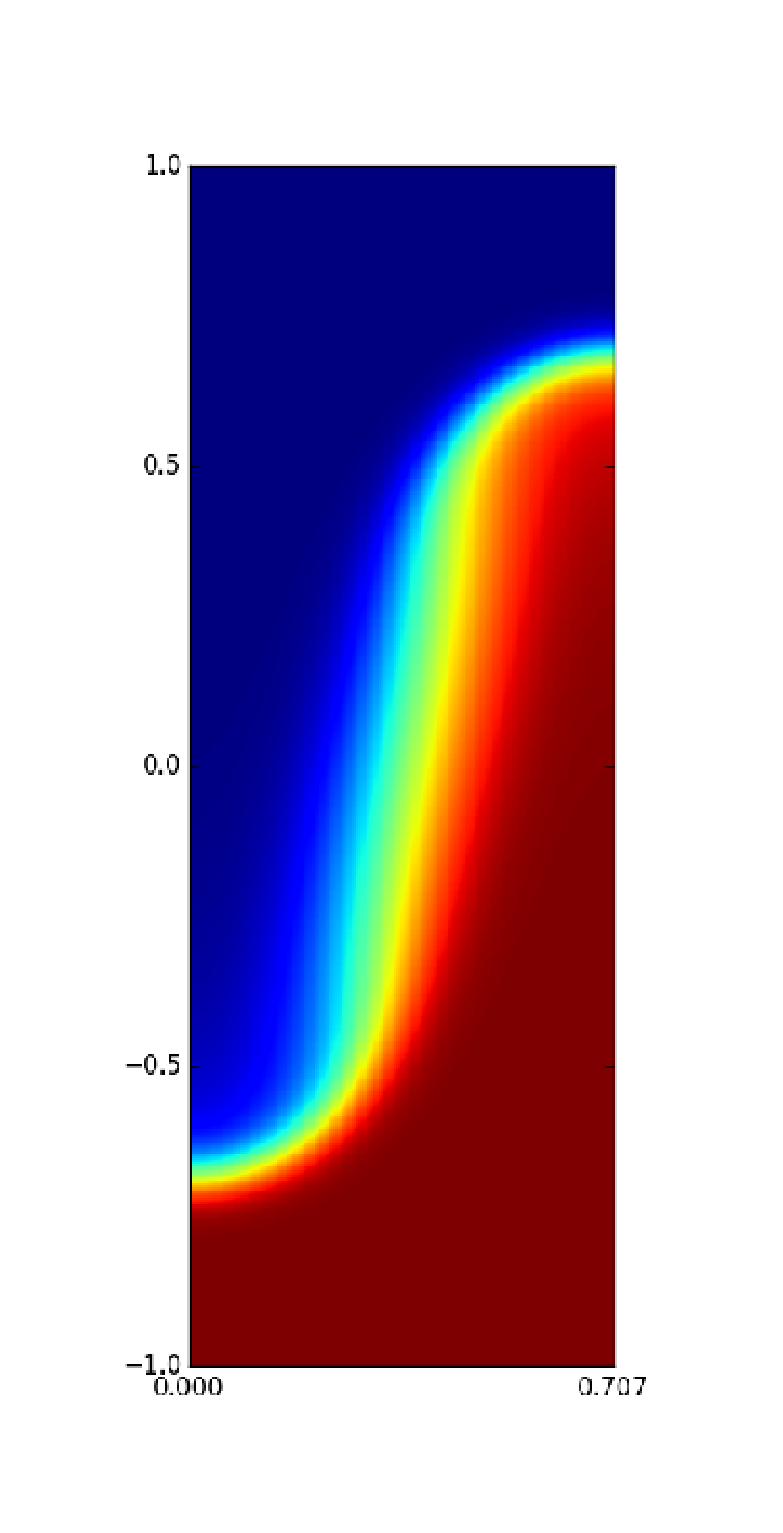
\includegraphics[width=\textwidth]{gfx/cnv_o16_e32-t_yz-0033}
\end{subfigure}
\begin{subfigure}[b]{0.24\textwidth}
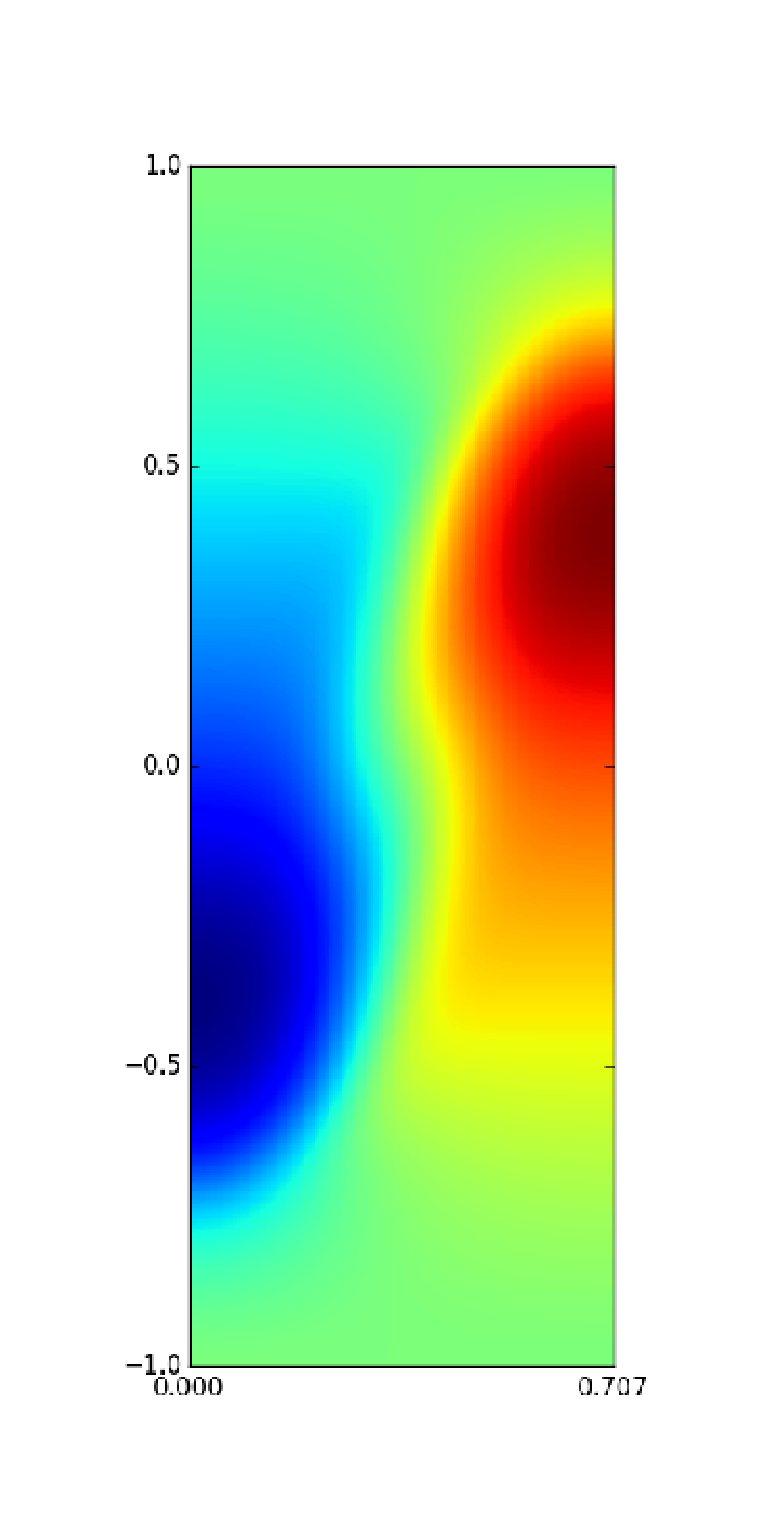
\includegraphics[width=\textwidth]{gfx/cnv_o16_e32-w_yz-0033}
\end{subfigure}
\begin{subfigure}[b]{0.24\textwidth}
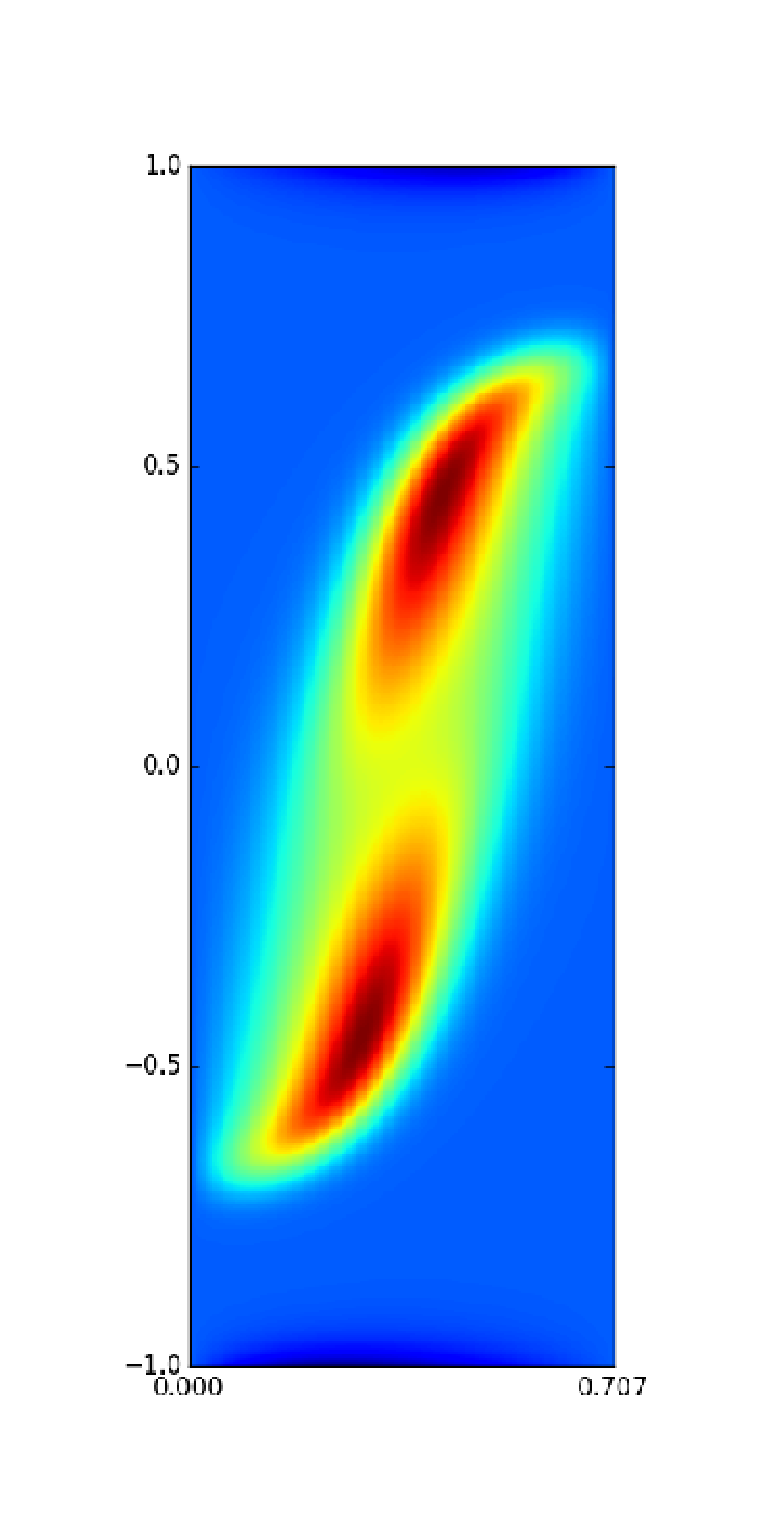
\includegraphics[width=\textwidth]{gfx/cnv_o16_e32-vorticity_yz-0033}
\end{subfigure}
\begin{subfigure}[b]{0.24\textwidth}
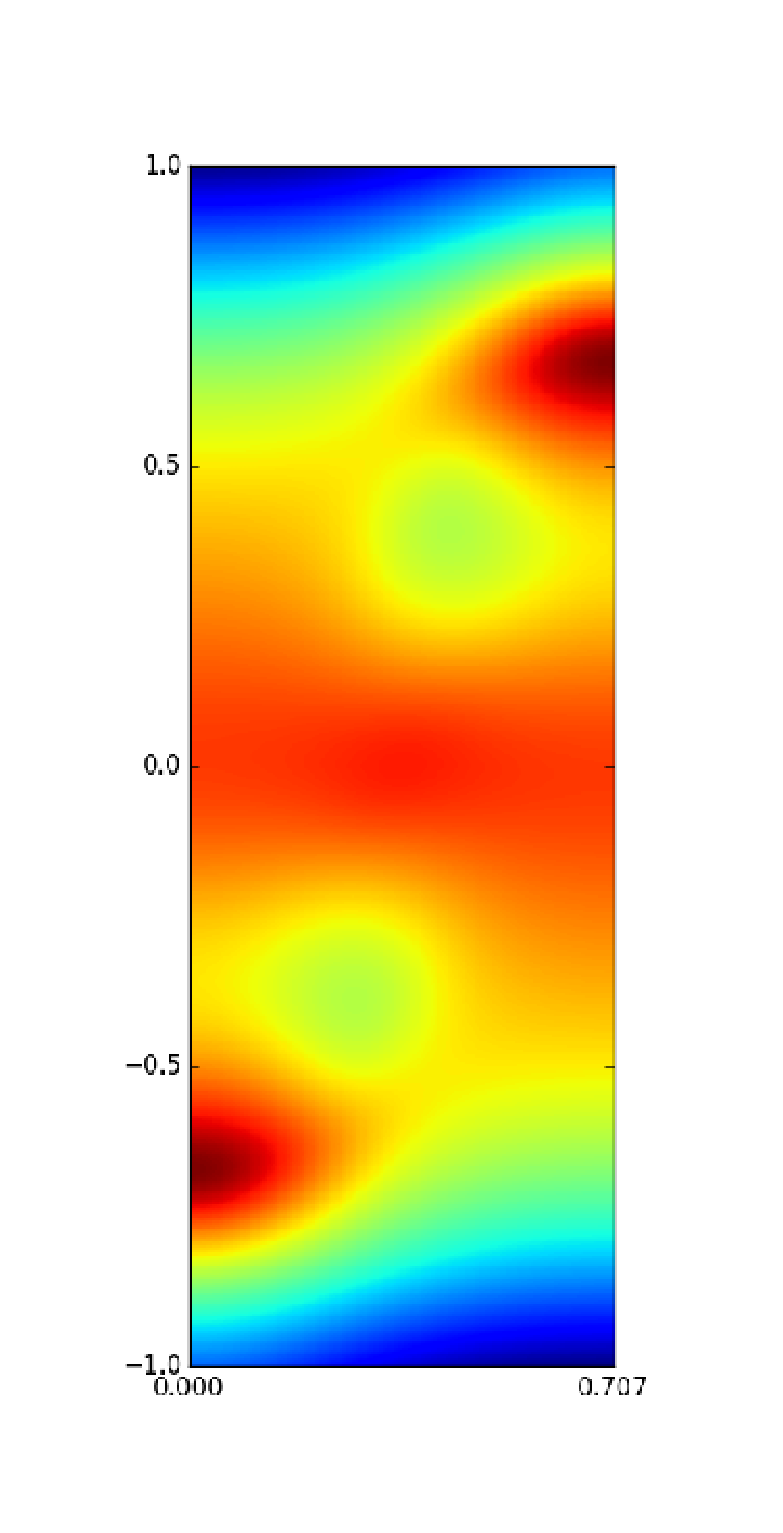
\includegraphics[width=\textwidth]{gfx/cnv_o16_e32-p_yz-0033}
\end{subfigure}
\caption{ \flabel{slices}
Scalar, vertical component of the velocity, vorticity component out of the plane, and pressure fields at end of simulation.
The color scales are dimensionless, linear, and centered at the mean value over the image.
}
\end{figure}

Slices of the end of the simulation are shown in \fref{slices}.
Two observables are calculated in post-processing: the \textit{bubble height} and the \textit{mix volume}:
\begin{equation} \elabel{observe}
H = \sup \left\{ z : \min_{x,y} ~ T(x,y,z) < T_0\right\}, \qquad
\Theta = \int \left|T - T_0\right| dV, 
\end{equation}
where $T_0$ is the volumetric average temperature.
These two observables are common to smRTI models and lie at opposite ends of the locality spectrum: 
the bubble height is defined by the neighborhood of the bubble tip while the mix volume is an integral over the entire domain.
The root mean square error in each observable is computed over all the outputs.


\subsection{Time to accuracy}

\begin{figure}
\begin{subfigure}[t]{0.49\textwidth}
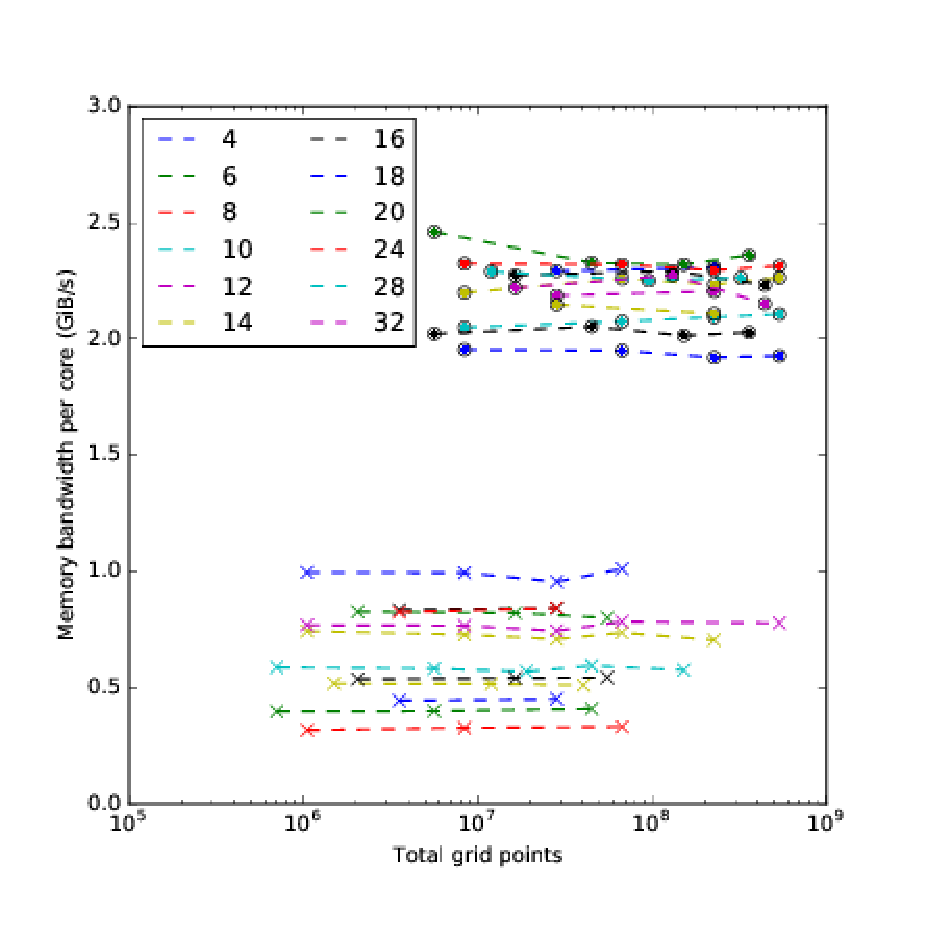
\includegraphics[width=\textwidth]{gfx/combined-bw}
\caption{Bandwidth}
\end{subfigure}
\begin{subfigure}[t]{0.49\textwidth}
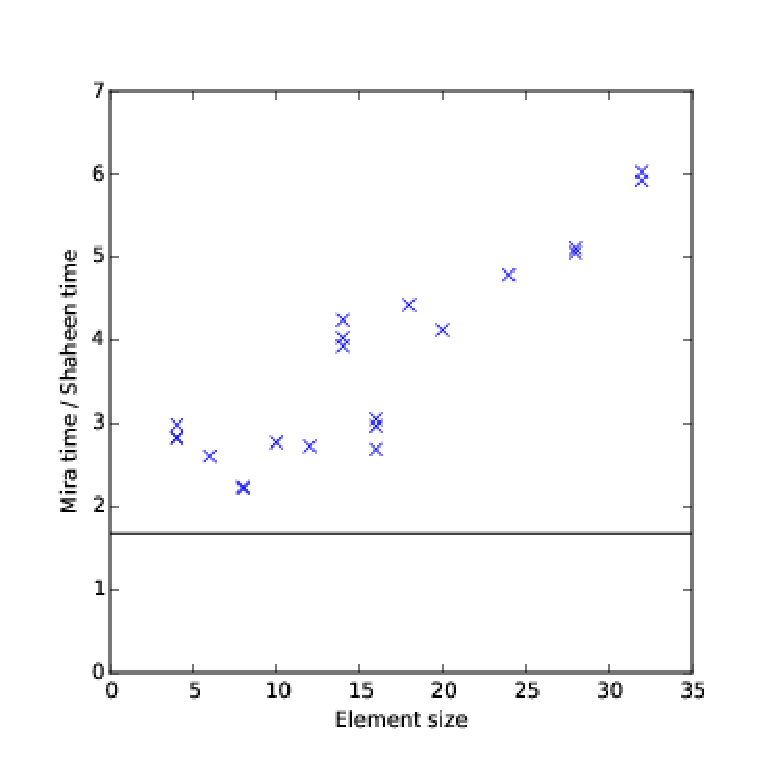
\includegraphics[width=\textwidth]{gfx/mira_vs_haswell}
\caption{Ratio}
\end{subfigure}
\caption{ \flabel{bwcomp}
Weak scaling of bandwidth on Shaheen and Mira.
In (a), Circles and crosses indicate memory bandwidth per core on Shaheen and Mira, respectively, vs.\ the problem size labeled by element size.
In (b), the ratio of the bandwidths are shown vs.\ element size for common discretizations.
The solid line indicates ratio of STREAM memory bandwidth.
}

\end{figure}

For each simulation, we compute the FLOP rate and aggregate memory bandwidth.
NekBox includes explicit FLOP and memory operation counters and timers in the most performance critical regions of the code.
Memory operations are counted assuming single-element intermediate data stays in cache, and therefore does not contribute to main memory bandwidth.
These counters are consistent with those used in the reproducers.
The whole application is not covered, so the counters can be considered lower bounds on the whole-application performance.

The attained memory bandwidth per core on Shaheen and Mira are plotted in \fref{bwcomp}.
On Shaheen, bandwidth is constant with respect to the number of elements and a weak function of the order, ranging from around 65 to 75\% of peak.
On Mira, bandwidth is still constant with respect to the scale, but varies more strongly with polynomial order, especially at orders greater than 16 and those not divisible by 4.
It ranges from around 15 to 50\% of peak.
The \texttt{mxm\_bgq} library, discussed in \sref{implementation}, is used, resulting in performance spikes at QPX-supported orders, e.g., 8.

\begin{figure}
\begin{subfigure}[t]{0.49\textwidth}
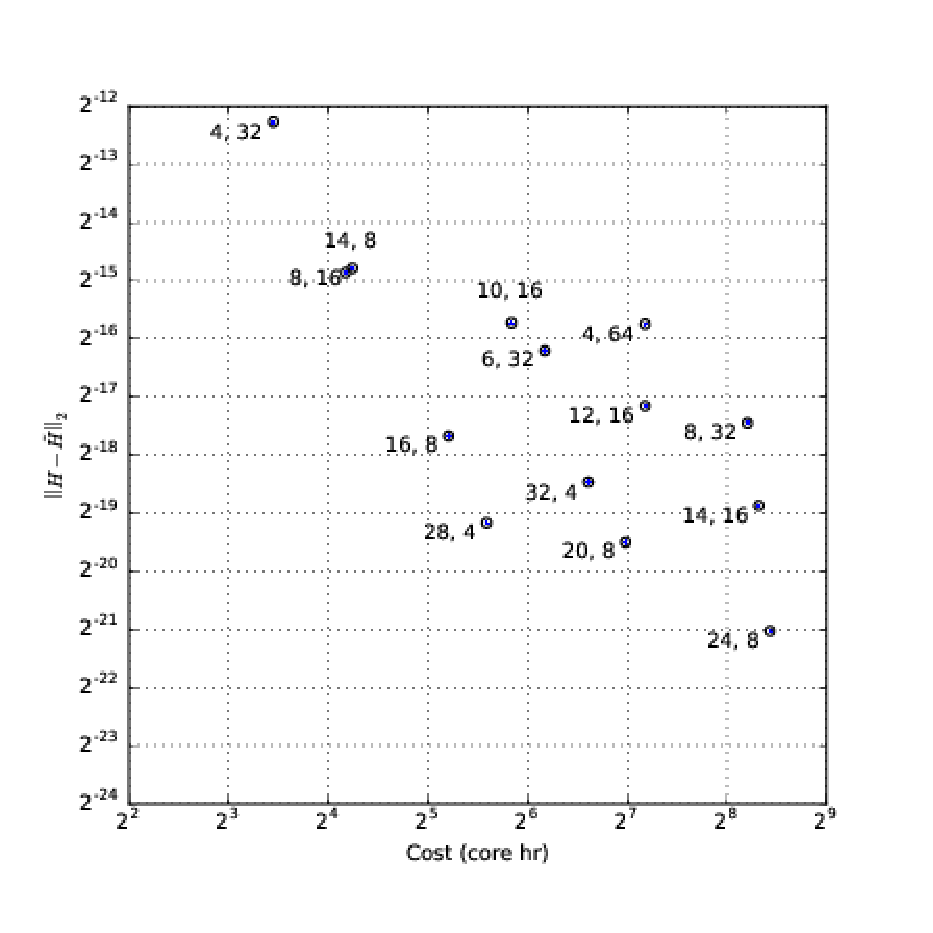
\includegraphics[width=\textwidth]{gfx/shaheen_H}
\caption{Shaheen}
\end{subfigure}
\begin{subfigure}[t]{0.49\textwidth}
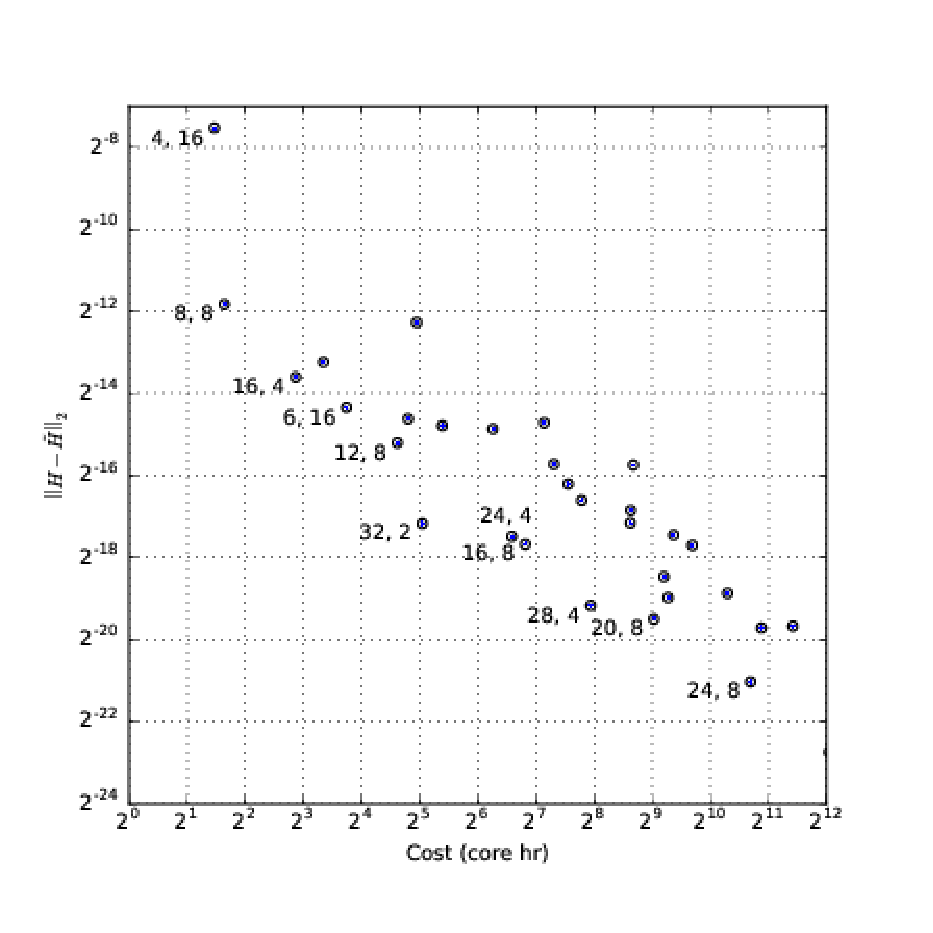
\includegraphics[width=\textwidth]{gfx/mira_H}
\caption{Mira}
\end{subfigure}

%\subfloat[][Error wrt $dt$]{\includegraphics[width=0.33\textwidth]{gfx/cnv_wrt_t}}
%\subfloat[][Shaheen ($\Theta$)]{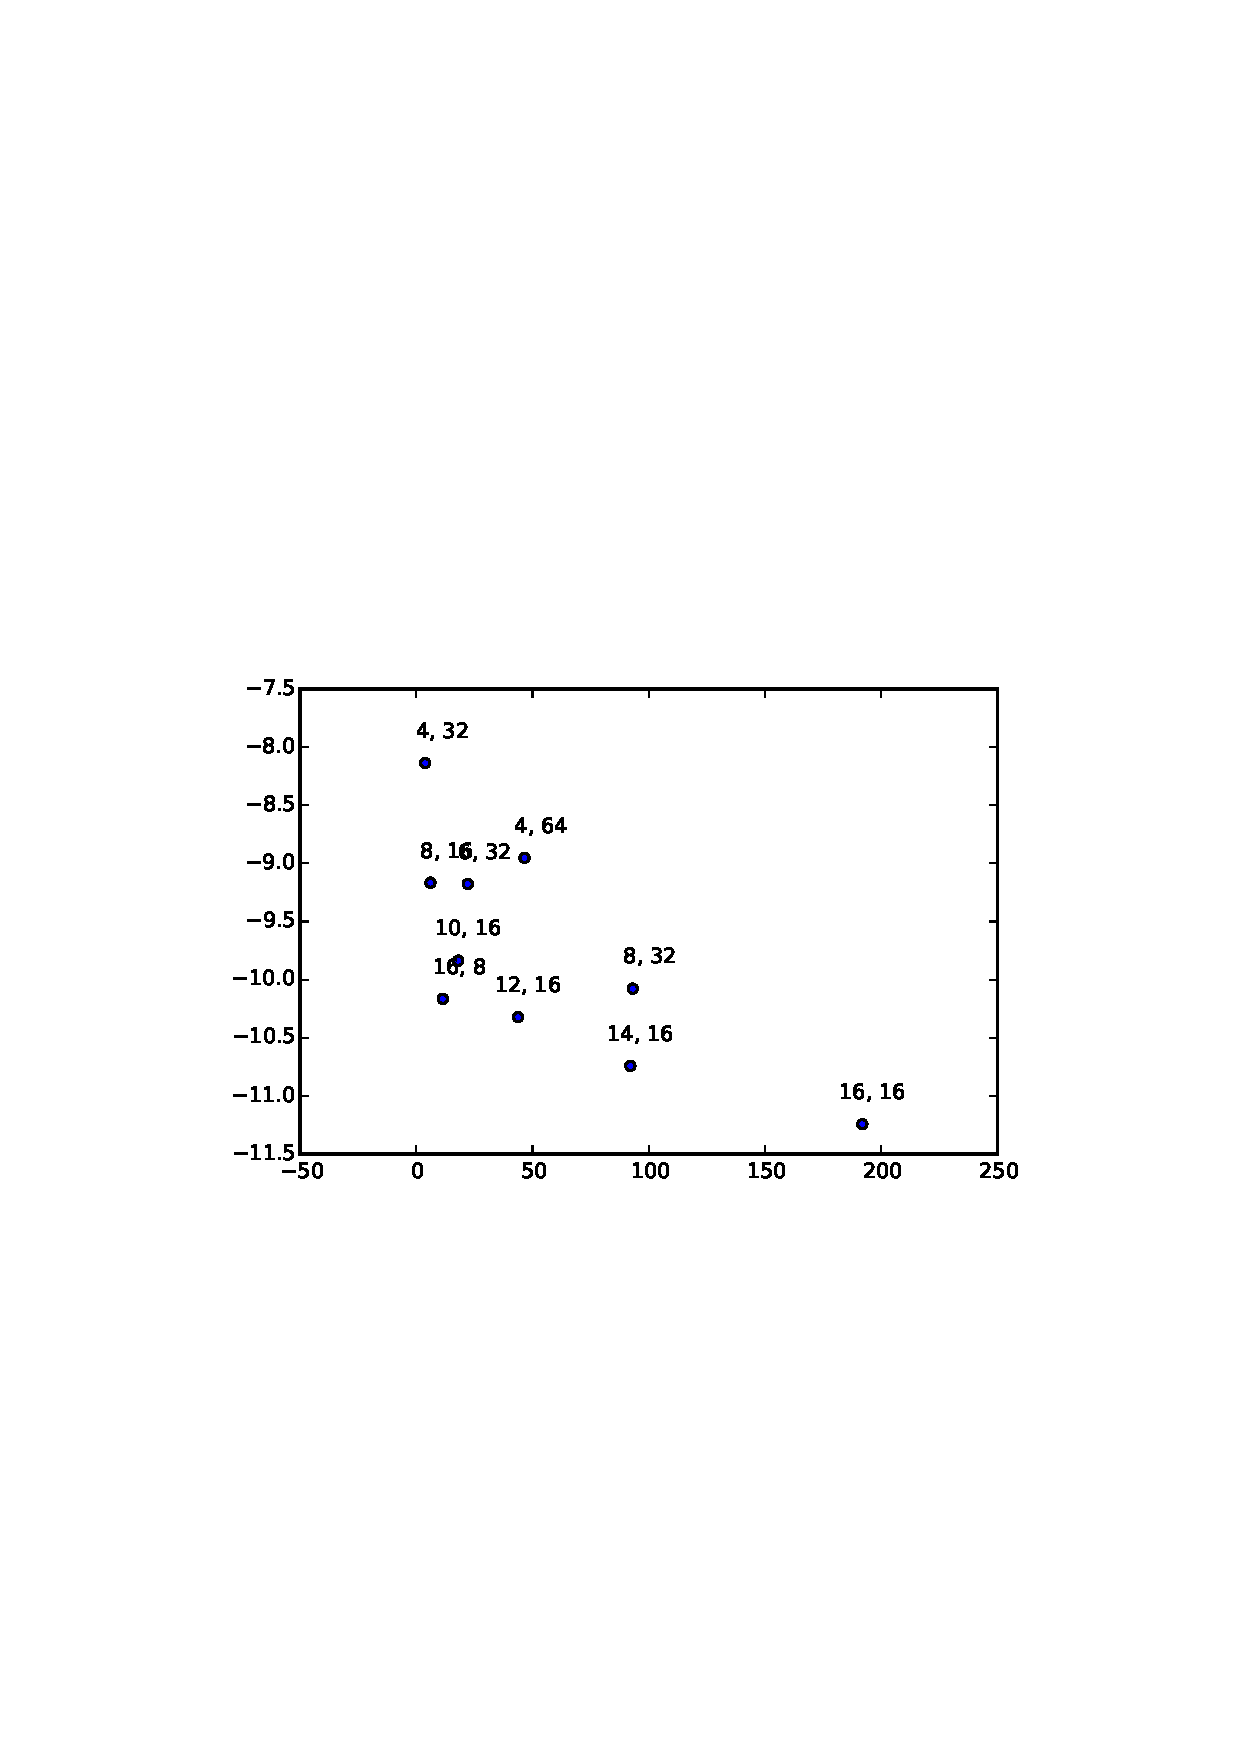
\includegraphics[width=0.5\textwidth]{gfx/shaheen_A}}

%\subfloat[][Mira ($\Theta$)]{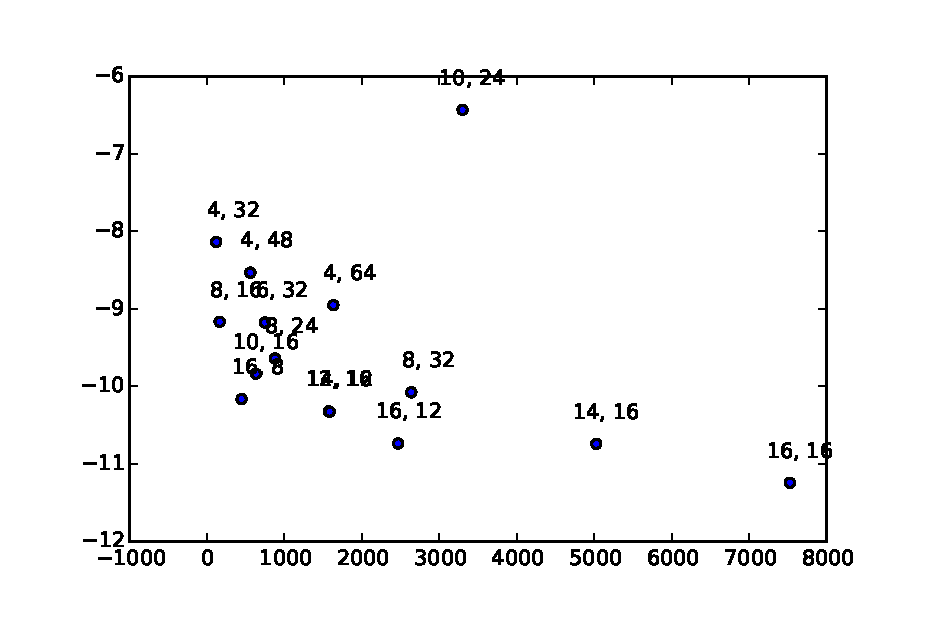
\includegraphics[width=0.5\textwidth]{gfx/mira_A}}

\caption{ \flabel{frontier}
Error with respect to bubble height, \eref{observe}, vs. the computational cost, in processor hours, on Shaheen (a) and Mira (b).
Points are labeled as $(p+1, e)$ pairs, where $p$ is the order, $p+1$ is the element size, and $e$ is the number of elements in one dimension.
More runs are present on Mira due to the smaller BGQ nodes evenly dividing more problem sizes.
}
\end{figure}

The accuracy is plotted versus the computational cost for a variety of discretizations in \fref{frontier}.
The error in bubble height and mix volume are strongly correlated, so only the error in the height is plotted.
As expected, doubling the the spectral order while keeping the number of elements fixed, e.g., $(4,32) \rightarrow (8,32)$ and $(8,8) \rightarrow (16,8)$, significantly improves the accuracy, but also increases the cost by 16-32$\times$.
The first 8$\times$ is due to an increase in the number of degrees of freedom, the next 2$\times$ is due to the shorter timestep, and, when compute-bound, the final 2$\times$ is due to an increase in the floating point load.
Doubling the spectral order while keeping the number of points fixed, e.g., $(16, 8) \rightarrow (32,4)$  and $(8,8) \rightarrow (16,4)$, increases the cost by 2-4x, as expected, but also improves the accuracy.
Doubling the spectral order while halving the number of points in each direction, e.g., $(8,32) \rightarrow (16,8)$ and $(14, 16) \rightarrow (28, 4)$, reduces the cost by 4-8$\times$ while maintaining or slightly improving the accuracy.

We define the \emph{efficiency frontier} as the set of discretizations that minimize computational cost for fixed accuracy or, equivalently, minimize error given fixed computational cost.
The efficiency frontiers on Mira and Shaheen are comprised of discretizations with very high orders, given our constraints.
The most efficient schemes are those with element size greater than 16, except for very low accuracy simulations.

\begin{comment}

\subsection{Order-independent timestepping}
\begin{figure}
\begin{subfigure}[t]{0.33\textwidth}
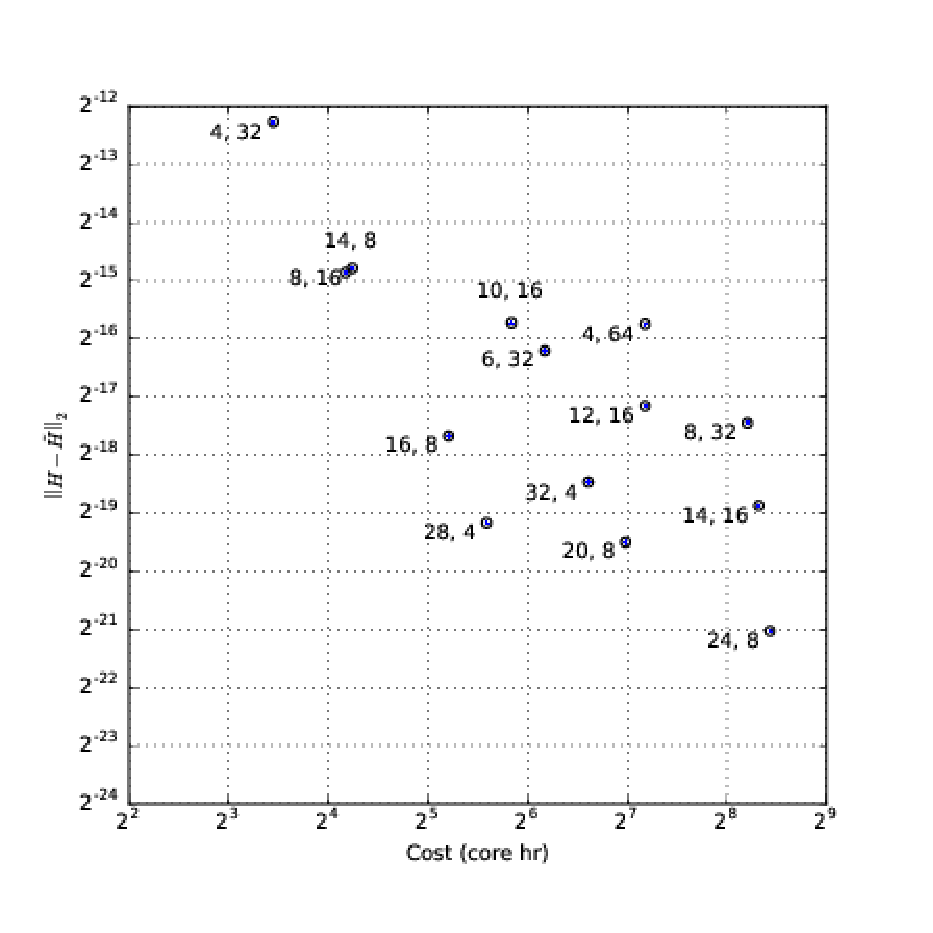
\includegraphics[width=\textwidth]{gfx/shaheen_H}
\caption{Shaheen}
\end{subfigure}
\begin{figure}
\begin{subfigure}[t]{0.33\textwidth}
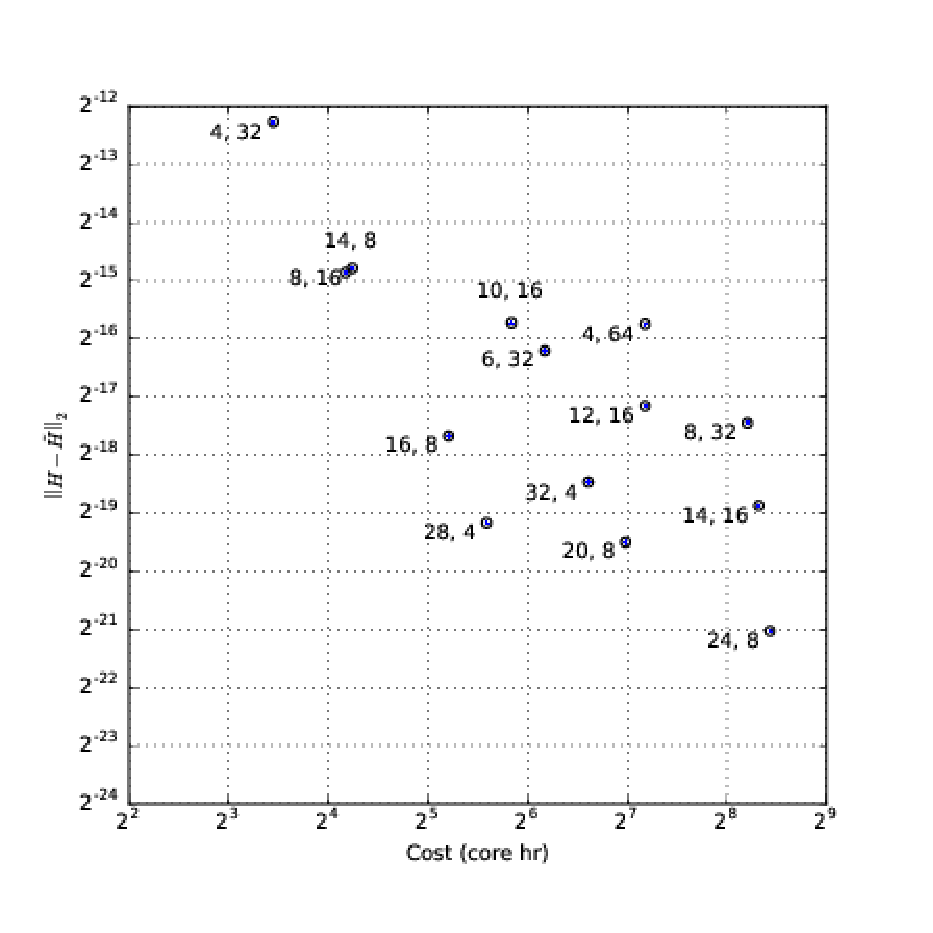
\includegraphics[width=\textwidth]{gfx/shaheen_H}
\caption{Mira}
\end{subfigure}
\begin{figure}
\begin{subfigure}[t]{0.33\textwidth}
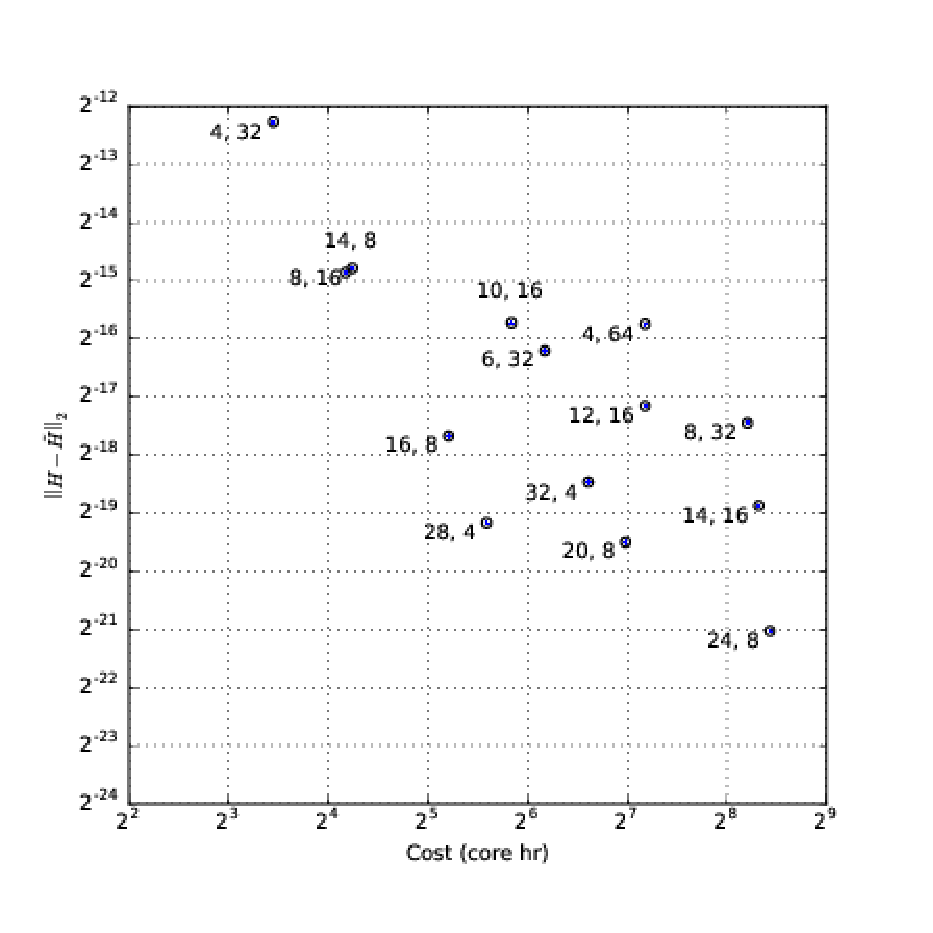
\includegraphics[width=\textwidth]{gfx/shaheen_H}
\caption{Cost vs DOF}
\end{subfigure}



	\subfloat[][Shaheen]{\includegraphics[width=0.33\textwidth]{gfx/shaheen_cfl_H}}
\subfloat[][Mira]{\includegraphics[width=0.33\textwidth]{gfx/mira_cfl_H}}
\subfloat[][Cost vs DOF]{\includegraphics[width=0.33\textwidth]{gfx/perf_vs_dof}}
%\subfloat[][Shaheen ($\Theta$)]{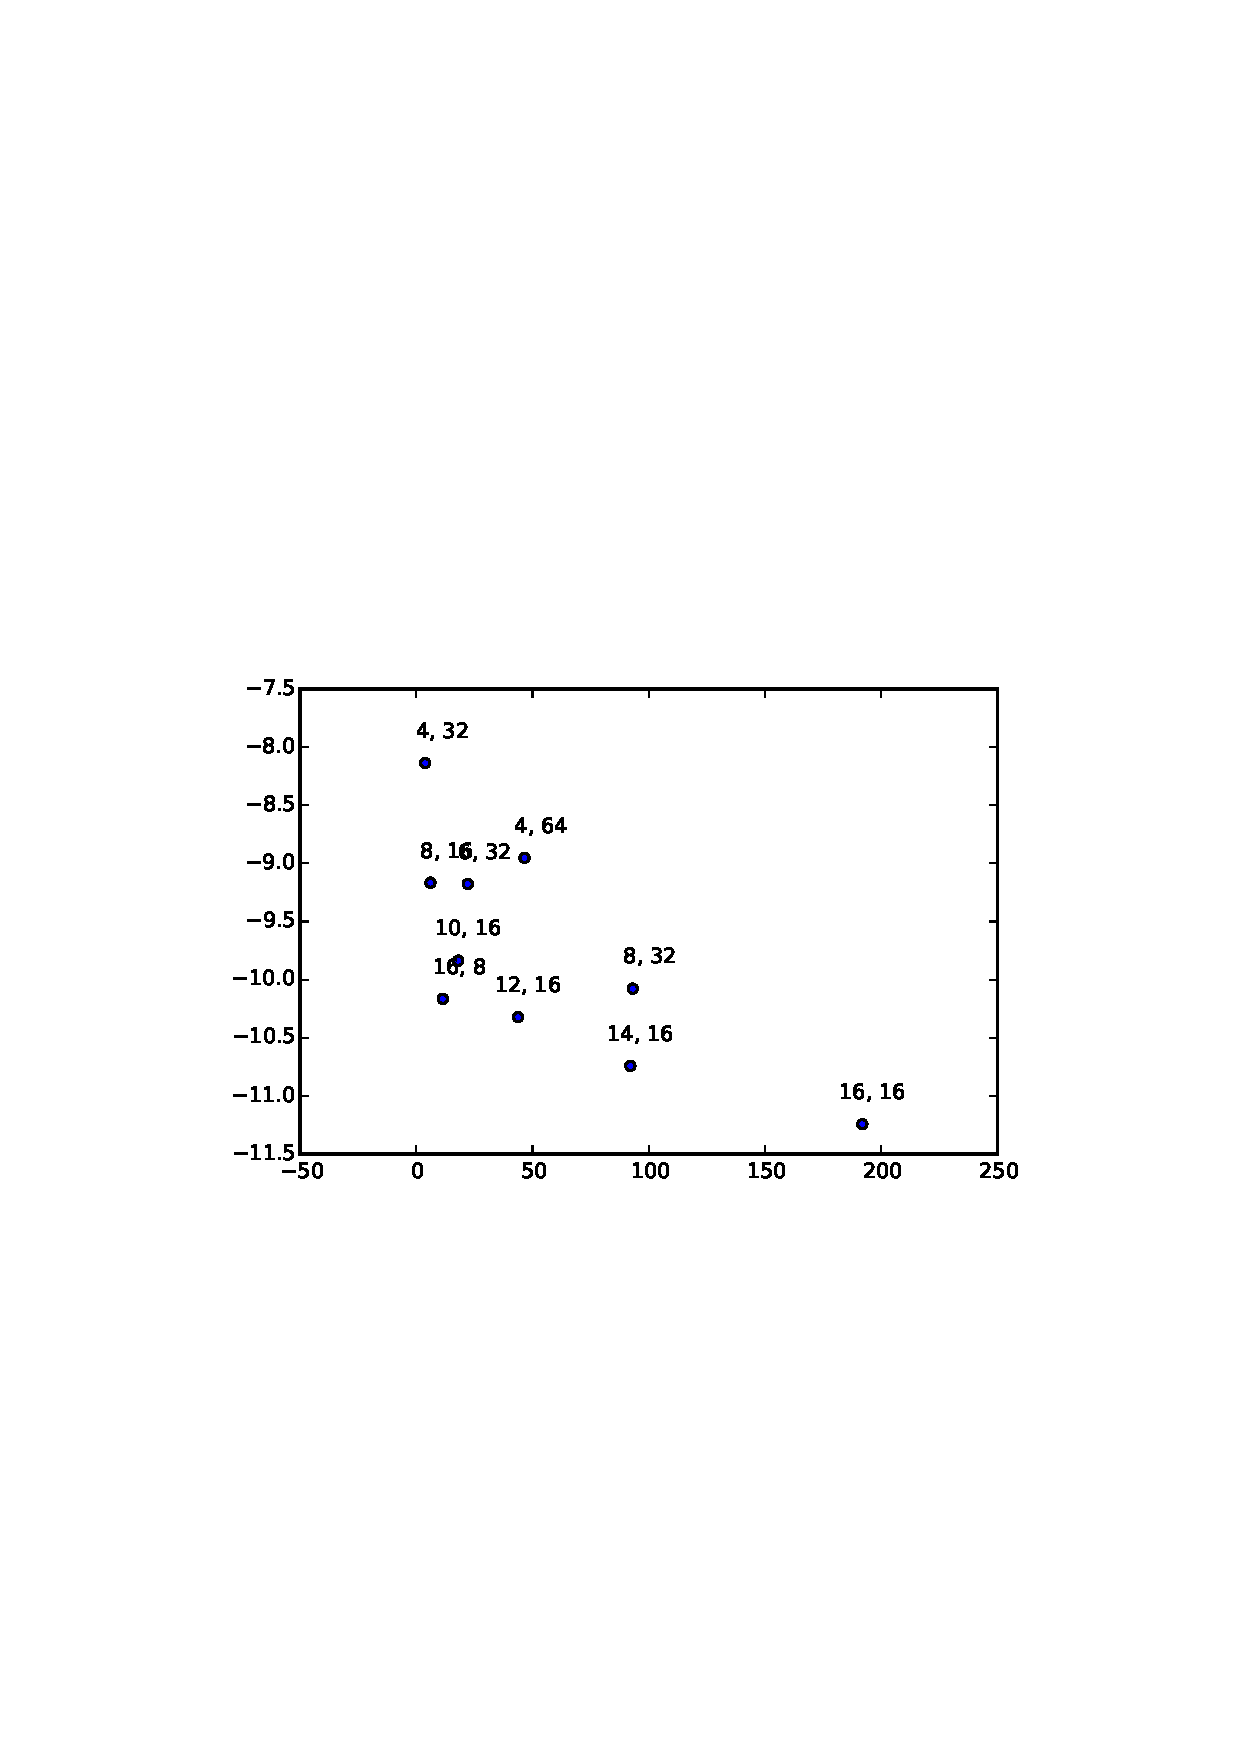
\includegraphics[width=0.5\textwidth]{gfx/shaheen_A}}

%\subfloat[][Mira ($\Theta$)]{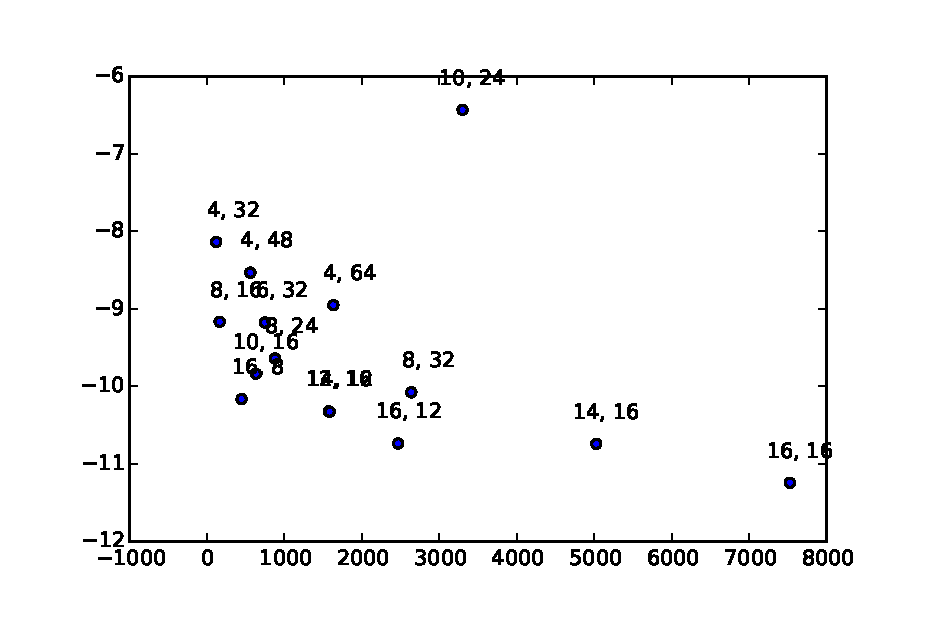
\includegraphics[width=0.5\textwidth]{gfx/mira_A}}

\caption{ \flabel{cfl3}
Error with respect to bubble height, \eref{observe}, vs. the computational cost, in processor hours, on Shaheen (a) and Mira (b).
Cost vs. total degrees of freedom (c), with circles from Mira and crosses from Shaheen.
In all cases, the ratio of timestep to maximal velocity is held fixed to match the CFL condition $C = 0.4$ in the (32,8) case, which sets the temporal error floor at the solid black line in (a) and (b).
}
\end{figure}

When using high order methods, there is often a gap between the convergence rate or the spatial and temporal discretizations.
To achieve high accuracy, it is necessary to reduce the timestep below the CFL stability condition.
Doing so decouples the number of timesteps from the element size.
Now, the computational cost depends on the order, for fixed total points, only through an increase in arithmetic intensity.
If the calculation is bandwidth-bound, then high order should come at no marginal cost.
If the calculation is compute-bound, then high order should come at linear cost, in return for exponential spatial convergence.

To demonstrate this, we reduce the time step to that of the $(32,8)$ discretization in the previous section by reducing the CFL number according to the spatial discretization.
This gives us a bound on the temporal error in $H$ of $2\times 10^{-6}$.
\fref{cfl3} plots the accuracy vs the computational cost, as in \fref{frontier} but with order-independent timestepping, along with the cost vs degrees of freedom.
We see that the most efficient calculations, those that minimize cost for a given error, are all very high order.
The cost is a strong function of the number of degrees of freedom and a weak function of the order.
On Shaheen in particular, the dependence of the cost on the order seems to be in the noise, all
runs took roughly the same computing time, independent from the chosen order.
\end{comment}

\begin{comment}
\subsection{Discussion}

\subsubsection{Time to solution}

Here, we have considered computational cost in the high-throughput context: the consumption of computational resources as measured in core hours.
Alternatively, one could consider the low-latency context: the minimum time to solution, i.e. the strong-scaling limit.
In this limit, we care about the number and computational duration of time iterations.

If we

This analysis can fail in at least three ways: a) we could saturate the network before we hit latency limits, which is unlikely given that Nek is predominantly nearest-neighbor; b) we could hit the coarse grain parallelism limit before we hit latency limits; or c) the number of iterations in the solvers could increase or decrease.

On low-latency networks, Nek5000's strong scaling limit is known to be of order 1000 grid points.
NekBox reduces the communication load, so its limit could be lower.
Therefore we expect to hit (b) at polynomial order between 10 and 16.
\end{comment}

\subsection{Whole application performance}

\begin{figure}[!t]
\centering
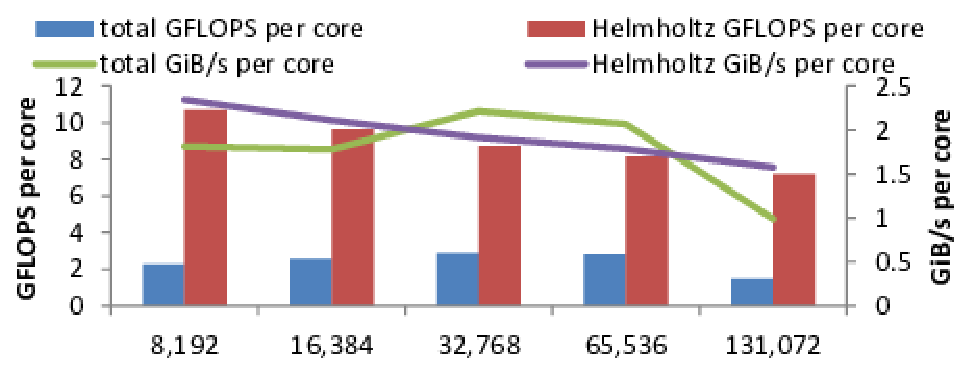
\includegraphics[width=0.55\textwidth]{gfx/shaheen_strong}
~
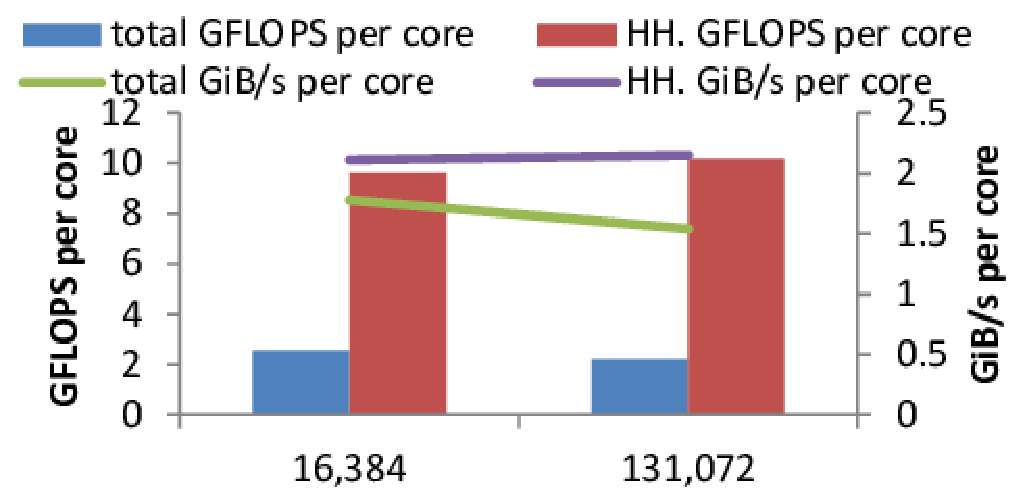
\includegraphics[width=0.42\textwidth]{gfx/shaheen_weak}
\caption{Strong scaling (left) and weak scaling (right) on Shaheen on up to 131,072  cores (2/3) of the full 7 PFLOPS machine using 
an element size of 32.
To avoid log plots we show per-core performance.}
\label{fig:shaheen_scaling}
\end{figure}

To date, our largest calculation on Shaheen occupied 131,072 cores, as depicted in Fig.~\ref{fig:shaheen_scaling}
for element size 32.
NekBox achieved 197 TiB/s memory bandwidth and 290 TFLOPS in weak scaling.
This corresponds to 47.8\% of peak memory bandwidth sustained over the entire application at high order.
In case of strong scaling these numbers are slightly lower with 130 TiB/s and 195 TFLOPS. 
%This is true for both, weak and strong scaling, as Shaheen uses dynamic  node-level power capping, that kicks 
%in when more than about 1/3 of the machine is used~\cite{pedretti2015early}. This cap is most likely caused by
%the high demand of compute and bandwidth of the Helmholtz as this phase is still scaling and achieves 
However, the Helmholtz operator, as the most compute intense sub-routine, is able to achieve
up to 0.94\,PFLOPS in strong and 1.33\,PFLOPS
 in weak-scaling on 131,072 cores. %\footnote{We are currently working together with KSL to root-cause the
%power capping issues. Due to the holidays this was not possible at submission deadline.}
We also consider 65,536 cores runs, occupying 1/3 of Shaheen.
These runs achieved at least 135.6 TiB/s memory bandwidth and 184.9 TFLOPS.
This corresponds to 67.5\% of peak memory bandwidth sustained over the entire application at high order.
Finally, extrapolating to full machine, NekBox would reach at least 406.8 TiB/s and 554.6 TFLOPS. At the same scale,
a weak scaling of the Helmholtz operator would result into 1.9\,PFLOPS out of 7\,PFLOPS performance.



